\chapter{The FlipIt game}
\label{cha:2}


\section{Extensions on FlipIt}


There a various possible ways to extend \flip{FlipIt}. For instance Laszka et al. extended the basic \flip{FlipIt} game to multiple resources. The incentive is that for compromising a system in a real case it needs more than just taking over one resource. An example is gaining access to a system and breaking the password. The model is called FlipThem \cite{FlipThem}. Two ways of flipping the resources are used: the AND and the OR control model. In the AND model the attacker only controls the system if he controls all the resources of the system, whereas in the OR model the attacker only needs to compromise one resource to be in control of the entire system. The difference with FlipThem and this paper is that we introduce a Graph Model in the beginning.\\
Another extension on FlipIt is done by Pham\cite{GameTheorApprCostBenefitAnalyses} [\todo{citatie needed voor Are We Compromised?}]. Beside the action Flip their is another action Test. The basic idea is to test with an extra action if the resource has been compromised or not. This action involves also an extra cost. This model is useful if somebody wants to know for example if his password has been compromised or wants to assess the periodic security of a system.  In \cite{MitigationCovert} \cite{MitigationNonTargeted} Laszka et al. they also consider non targeted attacks by non-strategic players and \todo{verder aanvullen}. 








In this section, we introduce the game \flip{FlipIt} \cite{FlipIt}. \flip{FlipIt} is a game introduced by .. .. and Rivest. First we explain the framework of FlipIt and after that the formulas and assumptions that we will make for the game for during the whole paper.  

\section{The First Topic of this Chapter}
\flip{FlipIt} is a two-players game with a shared (single) resource that the players want to control as long as possible. The shared resource can be a password, a network or a secret key depending on the setting being modelled. In the rest of the paper we will call the players the Attacker and the Defender. To get the control over the resource, players can flip the resource at any given time. Each move will imply a certain cost. The unique feature of \flip{FlipIt} is that the move will happen in a stealthy way, meaning that the other player has no clue that the other player has flipped the resource. For instance, the defender will not find out if the resource has already been compromised by the attacker, but he can only potentially know it after he flips the resource himself. The goal of the player is to maximize the time that he or she has control over the resource while minimizing total cost of the moves. Players won't move to frequently. A move can also result in a "wasted move", called a flop. It may happen that the resource was already under control by the defender. If the defender moves when he or she has already control over the resource, he or she would have wasted move since it does not result in a change of ownership. 
 
Because the players move in a stealthy way, there are different types of feedback that a player can get while moving:
\begin{itemize}
\item Non-adaptive (NA): The player does not receive any feedback while flipping.
\item Last move (LM): The player finds out the exact time the opponent played the last time.
\item Full History (FH): The player finds out the complete history of the opponents move.
\end{itemize}
The game can be extended by the amount of information that a player receives. It can also be possible for a player to get information at the start of the game. Both interesting cases are:
\begin{itemize}
\item Rate-of-play (RP: The player finds out the exact rate of play of the opponent.
\item Knowledge-of-strategy (KS): The player finds out the complete information of the strategy that the opponent is playing.
\end{itemize}

In our assumption the strategy of both players will be non-adaptive. None of the players has information of the strategy of the opponent. 



\section{Figures}
\begin{figure}[hbtp]
\centering
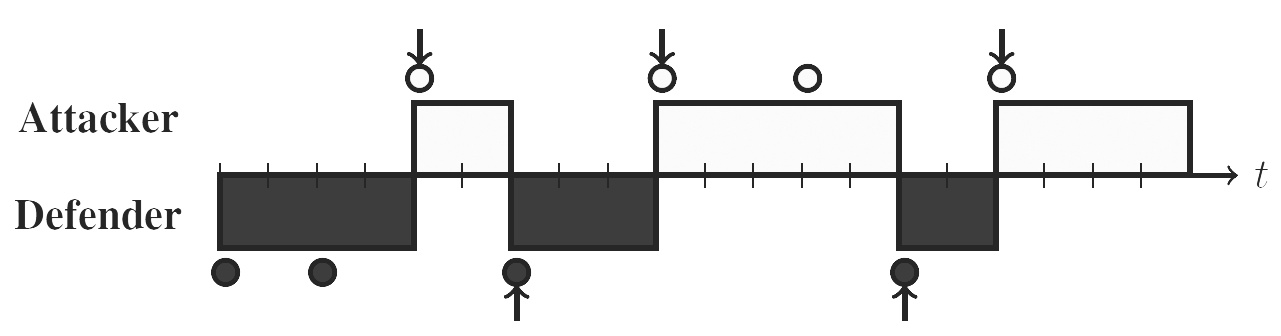
\includegraphics[scale=0.25]{Images/FlipItDefault.jpg}
\caption{The FlipIt game where both players are playing periodically}
\label{fig:FLipItDefault}
\end{figure}
\todo{verwijzen naar de figuur \ref{fig:FLipItDefault}}

\subsection{Strategies}
 
 In this subsection we go through the strategies used in FlipIt and the most important results. 
 \begin{table}
 \centering
 \begin{tabular}{ l | c  }
  \textbf{Categories} & \textbf{Classes of Strategies} \\
  \hline Non-adaptive (NA) & Exponential \\
  & Periodic \\
  & Renewal \\
  & General non-adaptive \\
  \hline Adaptive (AD) & Last move (LM) \\
  & Full History (FH) \\  
\end{tabular}
 \caption{Classes of strategies in FlipIt}
 \label{table:Strategies}
 \end{table}

There are two different kinds of strategies, the \textit{non-adaptive strategies} and the \textit{renewal strategies}. If there is no need for feedback for both of the players, we say that we have a non-adaptive strategy. Because the player does not receive any feedback during the game it will play in the same manner against every opponent. They are not dependent on the opponents movements. This means that they can already generate the time sequence for all the moves in advance.  But they can depend on some randomness because the non-adaptive strategies can be randomised. 
In this paper we will focus in the beginning on the non-adaptive strategies. Reasons behind this that a player (defender or attacker) rarely knows what the strategies are of his opponent. [If the attacker wants to move stealthily, it might have limited attack options FLIPTHEM]. \todo{nog redenen zoeken}\\
A renewal strategy is a non-adaptive strategy where the time intervals between two consecutive moves are generated by a renewal process. \\

 \begin{description}
 \item Periodic
 \item Non-Arithmetic Renewal
 \item Exponential
 \end{description}

\section{Formal definition Game}

In this section we provide the formal definition of the game and the notation that we will use throughout the paper.

\begin{description}
% ---- PLAYERS ---- %
\item \textit{Players}  There are two players in the game, one is the defender and the other one is the attacker. They are respectively identified by 0 and 1.

% ---- TIME ---- %
\item \textit{Time}  The game starts at $t=0$ and continuous indefinitely as $t \rightarrow \infty$. The game is a continuous game.

% ---- GRAPH ---- %
\item \textit{Graph} We represent the company network as a Graph $G = < V,E>$. G is an ordered pair where V denotes the set of resources or nodes in the network and E denotes the set of connections or links, which are a two-element subset of V. We use the notations resources and nodes interleaving in this paper.\\
We have N resources in the network. $N \in $  \todo{aanvullen}. This means we can denote the resources by:
\begin{center}
$V \in {V_{0}, V_{1}, V_{2}, ... , V_{N} }$
\end{center}
The set E of connections indicates if there is a link between two resources. We see the links as bidirectional so the total graph is undirected. If there is a link between resource $V_{n}$ and $V_{n+1}$ then there is also a link between $V_{n+1}$ and $V_{n}$. 

% ---- GAME STATE ---- %
\item \textit{Game State} There is also a time-dependent variable that represents the state of the game. $C=C(t)$ is either 0 if the game is under control by the defender and 1 if the Game is under control by the attacker. \\
We start at $t=0$ with the defender who has control over the game. We do this because we assume that the defender will only put the network online without having a virus or worm in it. The Attacker can gain control over the game when it compromises a subset \textit{s} of the resources. The subset \textit{s} is a minimum of 1 resource and a maximum of all the resources N. \\
\todo{deze variabele nodig ja of nee ? JA} We can also define the state of each resource by $C^{A}_{N}$ and $C^{D}_{N}$. If $C^{A}_{N} = 1$ then this means that the attacker has control over the resource, and 0 otherwise. For $C^{D}_{N}$ it is visa versa, $C^{D}_{N} = 1 - C^{A}_{N}$.\\

% ---- MOVES ---- %
\item \textit{Moves} Both players can make a move in the game. Moves done in a finite numbers of time in any finite time interval. Both players can play at any time they want, they can also play at the same time. If this happens the one that has control over the resource will keep having control over the resource.
This makes the game fully symmetric \todo{beter uitleggen}. The sequence of move times are denoted by the following infinite sequence:
\begin{center}
$t=t_{1},t_{2},t_{3},..$
\end{center}
Two move times can be the same because we allow players to move at the same time.
We can also denote the infinite sequence of times when player \textit{i}  moves. We write this as :
\begin{center}
$t=t_{i,1},t_{i,2},t_{i,3},..$ with \textit{i} $ \in $ $\lbrace 0,1 \rbrace$
\end{center}
The sequences $t_{1}$ and $t_{0}$ are disjoint subsets of the sequent t. 
We can also denote who made the \textit{k}th move by defining a sequence \textit{p} that denotes the sequence of who played:
\begin{center}
$p=p_{1},p_{2},p_{3}, .. $ with $p_{k}$ $\in$ $\lbrace 0,1 \rbrace$
\end{center}

% ---- NUMVER OF MOVES ---- %
\item \textit{Number of moves}  $n_{i}(t$ denotes the number of moves made by player \textit{i} up to and including time t. This means that 
\begin{center}
$n(t)=n_{1}(t) + n_{0}(t)$
\end{center}
is the sum of the number of moves made by the defender and the attacker up to and including time t. 

% ---- AVERAGE MOVE RATE ---- %
\item \textit{Average move rate} We denote $\alpha_{i}(t)$ as the average move rate by player i:
\begin{center}
$\alpha_{i}(t) = n_{i}(t)/t$ with $t > 0$ and \textit{i} $ \in $ $\lbrace 0,1 \rbrace$
\end{center}

% ---- PERIOD ---- %
\item \textit{Period} We can also define the period in terms of the average move rate:
\begin{center}
$\delta_{i}=1/\alpha_{i}$
\end{center}

% ---- WHO PLAYED LAST ---- %
\item \textit{Who played last} We know who played last by taking the modulo with the period. $Z_{i}$ represents the time since the last flip of player i. We can also denote the time since the last flip of player i on resource r by $Z_{i}^{N}$. 
For a non adaptive game, period deterministic: At time $t=n$ is $Z_{i} = n mod i$.  \todo{er kan nog steeds tegelijk geflipt zijn maar dan hebben ze wel geflipt}.


% ---- COST ---- %
\item \textit{Cost} The cost is an important property of the game. In FlipIt for every player the cost of a move is denoted by $k_{i}$. These costs can be very different for every player. In this game we denote the players flipping cost for resource $V_{N}$ by $c_{i}^{V_{N}}$. \\
For the defender the cost will be either the cost of flipping every resource or the cost of flipping a subgroup of the resources.\\
For the attacker the cost will be the cost of dropping a virus on a node. The spreading of the virus will not imply an extra cost. 

% ---- UTILITY/ GAIN ---- %
\item \textit{Utility} In FlipIt the Gain definition is the utility function. The Gain denotes the total time a player i has gained control over a resource. \todo{nu gain van een resource, moet voor verschillende resources zijn}
The Gain $G_{i}$ denotes players i total gain of a game, wich is the total time the player has gained control over a subset of resources thus controlling the game. If we sum up the total Gain of the attacker and the defender we end up with the time:
\begin{center}
$G_{1}(t) + G_{0}(t) = t$
\end{center}

% ---- AVERAGE GAIM RATE ---- %
\item \textit{Average gain rate} The average gain rate for player i is defined as
\begin{center}
$\gamma_{i}(t)= G_{i}(t)/t$
\end{center}

\subsection{Our Game parameters}
\begin{description}
\item \textit{Graph Matrix} We represent the graph of the network through a matrix $ A = |V| \times |V|$. The (i,j)-entry of the matrix A will have a 1 if there is a connection between node $V_{i}$ and node $V_{j}$. If we are working with an undirected graph the matrix will be symmetric. 
\item \textit{Attack Vector} We denote $X = 1 \times |V|$ as the attack vector.  
\item \textit{Reset vector} The reset vector will make sure that the right entries in the matrix become zero.
\item \textit{Cummulative Matrix} 
\item \textit{State Matrix} The State matrix $T(t) = |V| \times |V| $ will keep at every time t the state of the game.
\end{description}

\end{description}


\section{Conclusion}
The final section of the chapter gives an overview of the important results
of this chapter. This implies that the introductory chapter and the
concluding chapter don't need a conclusion.



%%% Local Variables: 
%%% mode: latex
%%% TeX-master: "thesis"
%%% End: 
